\documentclass{report}

% Packages
\usepackage[utf8]{inputenc}
\usepackage[T1]{fontenc}
\usepackage{lipsum} % for dummy text
\usepackage[english]{babel}
\usepackage{csquotes}
\usepackage{amsmath}
\usepackage{amsfonts}
\usepackage{hyperref}

\edef\restoreparindent{\parindent=\the\parindent\relax}
\usepackage{parskip}
\restoreparindent

\usepackage{algorithm,algpseudocode}

\newcommand\independent{\protect\mathpalette{\protect\independenT}{\perp}}

\usepackage{amsthm}
\newtheoremstyle{slanted}%
  {12pt}   % Space above
  {12pt}   % Space below
  {\itshape} % Body font
  {}       % Indent
  {\bfseries} % Head font
  {.}      % Punctuation after theorem head
  { }      % Space after theorem head
  {}       % Head spec

\theoremstyle{slanted}
\def\independenT#1#2{\mathrel{\rlap{$#1#2$}\mkern2mu{#1#2}}}
\newtheorem{theorem}{Theorem}[section]
\newtheorem{definition}{Definition}[section]
\newtheorem{lemma}{Lemma}[section]
\newtheorem{proposition}{Proposition}[section]
\newtheorem{corollary}{Corollary}[section]
\newtheorem{remark}{Remark}[section]

% tikz
\usepackage{tikz}
\usetikzlibrary{decorations.pathreplacing}
\usetikzlibrary{calc}
\usetikzlibrary {bending,positioning}

%
\def\cl#1{\centerline{#1}} \def\eqcl#1{\cl{$\displaystyle#1$}} \def\eq#1{{$\displaystyle#1$}}

\def\nablab{\text{\boldmath$\nabla$}}
\def\wh#1{\widehat{#1}}    \def\wt#1{\widetilde{#1}}
%\def\foo#1{{\text{\def\scad{-3}\tiny #1}}}
\def\foo#1{\textrm{#1}}
\def\T{^\tD}
%\def\T{^T}
\def\M{^{-1}}
\def\MT{^{-\tD}}
\def\+{^\dagger}
\def\I{\,|\,}           % "sachant" bien espacé pour les formules
\def\J{\mathop{\,;\,}}  % "point virgule" bien espacé pour les formules.
\def\w{,\thinspace}
\def\W{,\thickspace}
\def\ldotsv{,\,\ldots,\,}
\def\Exp#1{\exp\acc{#1}}
\def\Expp#1{e^{#1}}
\def\argmax{\mathop{\mathrm{arg\,max}}} % Mieux que \def\argmax{\arg\max}
\def\argmin{\mathop{\mathrm{arg\,min}}} % car l'indice est reparti
\def\Vect{\mathop{\text{Vect}}}
\def\Card{\mathrm{Card}}
\def\Circul#1{\mathrm{Circul}\{#1\}}
\def\toeplitz#1{\mathrm{T{\oe}plitz}\{#1\}}
\def\Id{\mathit{Id}}
\def\cste{\mathrm{cste}}
\def\tr{\mathrm{tr}}
\def\rang{{\mathrm{rang}}}
\def\Cov{\mathrm{Cov}}
\def\diag{{\mathrm{diag}}}
\def\Diag{\mathrm{Diag}}
\def\DIAG#1{\mathrm{Diag}\acc{#1}}
\def\Ker{\mathrm{Ker\,}}
\def\Img{\mathrm{Im\,}}
\def\Div{{\mathrm{div}}}
\def\FT#1{\protect\accentset{\frown}{#1}}
% Pour mettre un \No{} au-dessus d'une lettre (\TM, 02/97) (package{amsmath.sty})
%\def\rond#1{\overset{\kern-0.33em~_\circ}{#1}}
%\def\rondit[#1]#2{\overset{\kern#1~_\circ}{#2}}
\def\EL{\mathrm{EL}}
\def\esp{\ED\,}
\newcommand{\Esp}[2][]{\ED{_{#1}}\kern-2pt\cro{#2}}
%\def\Esp#1{\ED\kern-1pt\pth{#1}}
\def\stdEsp#1{\ED\stdcro{#1}}
%\def\EMQ{\mathit{EMQ}}
\def\var{\mathrm{var}\,}	\def\Var#1{\mathrm{var}\pth{#1}}	
\def\cov{\mathrm{cov}}		\def\Cov#1{\mathrm{cov}\kern-2pt\pth{#1}}
\def\egal{\kern-.5em=\kern-.5em}
\def\egdef{\stackrel{\Delta}{=}}
\newcommand{\imag}[1]{\mathrm{Im}\acc{#1}}
\newcommand{\reel}[1]{\mathrm{Re}\acc{#1}}
\newcommand{\impur}{\ensuremath{j}}

\def\sump{\mathop{\raisebox{-.3ex}{\text{\Large$\Sigma$}}}}
\def\intp{{\text{\small$\int$}}}
\def\prodp{\mathop{\raisebox{-.3ex}{\text{\Large$\Pi$}}}}
\newcommand{\fracp}[2]{\frac{\raisebox{-1pt}{$#1$}}{#2}}
\newcommand{\UNsur}[1]{\fracp{1}{#1}}
\def\demi{\UNsur{2}}
\def\ds{\displaystyle}
\def\ss{\scriptstyle}
\def\fracds#1#2{{\ds\frac{#1}{#2}}}
\def\fracts#1#2{{\ss\frac{#1}{#2}}}
\def\derpar#1#2{{\frac{\partial #1}{\partial #2}}}
\def\froc#1#2{{#1/#2}}     \def\fric#1#2{\frac1{#2}#1}
\def\derpor#1#2{{\froc{\partial #1}{\partial #2}}}
\def\parsec#1#2#3{{\frac{\partial^2 #1}{\partial #2\,\partial #3}}}
\def\parsecd#1#2{{\frac{\partial^2 #1}{{\partial #2}^2}}}
\def\porsec#1#2#3{{\froc{\partial^2 #1}{\partial #2\,\partial #3}}}
\def\porsecd#1#2{{\froc{\partial^2 #1}{{\partial #2}^2}}}
\def\pornd#1#2#3{{\froc{\partial^{#3} #1}{{\partial #2}^{#3}}}}
%\def\sur{\ensuremath{\kern-1pt/\kern-1pt}}
\def\diff#1#2{{\frac{\dd#1}{\dd#2}}}

% Bibliography setup
\usepackage[backend=biber,style=authoryear,maxnames=1]{biblatex}

\DeclareCiteCommand{\cite}
  {\usebibmacro{prenote}}
  {\printtext[bibhyperref]{%
     [\printnames{labelname}~\printfield{year}]}}
  {\multicitedelim}
  {\usebibmacro{postnote}}

\DeclareDelimFormat{multicitedelim}{\addcomma\space}

\addbibresource{reference/PET.bib}
\addbibresource{reference/PnP.bib} % name of your .bib file (explicit path so biber finds it when building from workspace root)
\addbibresource{reference/optimisation.bib}
\addbibresource{reference/Self-supervised.bib}
\addbibresource{reference/denoising.bib}

%
\usepackage{indentfirst}
\usepackage[a4paper, total={6in, 8in}]{geometry}



\title{PhD Bibliography : Optimization of learning-based methods without ground truth and applicability to positron emision tomography}
\author{Sacha Bouchez-Delotte}
\date{\today}

\begin{document}



\maketitle

\newpage
\tableofcontents
\newpage

\begin{abstract}
This doctoral project aims at proposing new statistical learning based methods to solve linear inverse problems, and more specifically image reconstruction. The focus will be laid on the possibility to perform the training stage without ground truth images, provided that suited sets of noisy data are available, as pioneered by the authors of Noise2noise. A second step of the project will be to consider Positron Emission Tomography (PET) imaging as a specific application case, in collaboration with Nantes CHU. In this context, list mode data can be split into statistically independent subsets in many ways, which could yield a tailored version of Noise2noise with enhanced properties.
\end{abstract}

\newpage

\chapter{General introduction}

\section{Introduction to linear inverse problems}

The main focus of this section is to present mathematical inverse problems, which are problems where we aim to recover an underlying signal from indirect and noisy measurements. These problems are common in various fields such as image reconstruction, signal processing, and machine learning.
We limit ourselves to linear inverse problems in finite dimensions. This allows us to derive theoretical results and develop efficient algorithms for solving these problems.

Let $(\Omega, \mathcal{F}, \mathbb{P})$ be a probability space and $X: \Omega \to \mathcal{X}$ a random variable representing the true signal. We assume that we have access to measurements $Y: \Omega \to \mathcal{Y}$ that are related to the true signal through a linear operator $A: \mathcal{X} \to \mathcal{Y}$ and corrupted by a noise process $\mathcal{C}$. The measurement model can be written as:
\begin{equation}
    Y | X=x \sim \mathcal{C}(Ax)
    \label{eq:inverse-problem}
\end{equation}

In most setups, we work in high dimensions and the forward operator $A$ is not directly invertible, which makes the problem of recovering $X$ from $Y$ an ill-posed inverse problem.

\begin{definition}
    $A$ is said to be ill-posed if one of the following properties is not satisfied :
\begin{enumerate}
    \item $A$ is injective, i.e. $\forall x_1, x_2 \in \mathcal{X}, Ax_1 = Ax_2 \implies x_1 = x_2$.
    \item $A$ is surjective, i.e. $\forall y \in \mathcal{Y}, \exists x \in \mathcal{X}$ such as $y = Ax$.
    \item $A^{-1}$ is continuous, i.e. $\forall \epsilon > 0, \exists \delta > 0$ such as $\| y_1 - y_2 \| < \delta \implies \| A^{-1}y_1 - A^{-1}y_2 \| < \epsilon$.
\end{enumerate}
\end{definition}

\begin{remark}
    Note that in finite dimention, linear bijections are always continuous and thus the third condition is automatically satisfied.
\end{remark}

If $A$ is ill-posed, then it is obviously not a bijection and its null-space is not reduced to $\{0\}$.
This means that there exist many solutions to the inverse problem for a given measurement, eventhough we're looking for a unique solution.


\begin{definition}{Minimal-norm solution}
    \begin{enumerate}
    \item $x \in \mathcal{X}$ is a least-squares solution if 
    \begin{equation*}
        \| Ax - y \| = \inf_{z \in \mathcal{X}} \| Az - y \|
    \end{equation*}
    \item $x \in \mathcal{X}$ is a minimal-norm solution if it is a least-squares solution and $\| x \| = \inf_{z \in \mathcal{X}, Az = y} \| z \|$.
    \end{enumerate}
\end{definition}

% \begin{definition}{Convergence of solution sequence}
%     Let $(y_\delta)_{\delta > 0}$ be a sequence of measurements such that $\| y_\delta - y \| \leq \delta$.
%     This sequence is said to be convergent with regard to an inverse operator $A^\dagger$ if the sequence of minimal-norm solutions $(x_\delta)_{\delta > 0}$ defined by $x_\delta = A^\dagger y_\delta$ converges to the minimal-norm solution $x^\dagger$ of $y$, i.e. $\lim_{\delta \to 0} \| x_\delta - x^\dagger \| = 0$.

% \end{definition}


\begin{proposition}
    If $A \in \mathcal{L}(\mathcal{X}, \mathcal{Y})$ is a bounded operator and if a least square solution exists, then the minimal-norm solution is unique and is given by $ x ^\dagger = A^\dagger y$ where $A^\dagger$ is the Moore-Penrose pseudo-inverse of $A$. \cite{sherry2025part}
\end{proposition}

\subsection{Regularisation of inverse problems}

If the range of $A$ is not closed, then Moore-Penrose pseudo-inverse may not be well-posed.
Thus, given noisy data $y_\delta$ such that $\| y_\delta - y \| \leq \delta$, the least-squares solution $A^\dagger y_\delta$ may not converge to the minimal-norm solution $x^\dagger$ as $\delta \to 0$.
This is the reason why we need to replace $A^\dagger$ with a family of well-posed and bounded operators $(R_\alpha)_{\alpha > 0}$, called regularisation operators, that approximate $A^\dagger$ as $\alpha \to 0$, hence the following definition.

\begin{definition}{Regularisation}
    A family of continuous operators $(R_\alpha)_{\alpha > 0}$ is called a regularisation of $A^\dagger$ if $\lim_{\alpha \to 0} R_\alpha y = A^\dagger y$ for all $y \in \mathcal{Y}$.
\end{definition}

$\alpha$ is called the regularisation parameter. Setting it to a small value allows us to get a good approximation of the minimal-norm solution, but it also makes the regularisation operator more sensitive to noise. On the other hand, setting $\alpha$ to a large value makes the regularisation operator more robust to noise, but it also leads to a worse approximation of the minimal-norm solution. Therefore, choosing an appropriate value for $\alpha$ is crucial for obtaining good reconstruction results.
This can be seen thanks to the following observation :
\begin{equation*}
    \begin{aligned}
        \| R_\alpha y_\delta - x^\dagger \| &\leq \| R_\alpha y_\delta - R_\alpha y \| + \| R_\alpha y - A^\dagger y \| \\
        & \leq \delta \| R_\alpha \| + \| R_\alpha y - A^\dagger y \|
    \end{aligned}
\end{equation*}
where the first term is some noise amplification term and the second term is some approximation error term. The first term is increasing with $\alpha$ while the second term is decreasing with $\alpha$, which means that there is a trade-off between noise amplification and approximation error when choosing $\alpha$.
This decomposition also indicates that the regularisation parameter $\alpha$ should be chosen according to the noise level $\delta$ in order to achieve a good reconstruction performance.

\subsubsection{Parameter choice rule}

\begin{definition}{Parameter choice rule}
    A parameter choice rule is a function $\alpha: \mathbb{R}^+ \times \mathcal{Y} \to \mathbb{R}^+ \mapsto \alpha(\delta, y_\delta)$.
    There are three parameter choice rule families :
    \begin{itemize}
        \item A priori parameter choice rule : $\alpha$ depends only on $\delta$.
        \item A posteriori parameter choice rule : $\alpha$ depends only on $y_\delta$.
        \item Heuristic parameter choice rule : $\alpha$ depends on both $\delta$ and $y_\delta$.
    \end{itemize}
\end{definition}


In this case, we can still define the minimal-norm solution as the limit of the least-squares solutions for a sequence of measurements that converges to $y$ :

\begin{equation*}
    x^\dagger = \lim_{\delta \to 0} A^\dagger y_\delta
\end{equation*}

\subsection{Spectral regularisation}

\subsubsection{Operator compactness}

\begin{definition}
    An operator $A \in \mathcal{L}(\mathcal{X}, \mathcal{Y})$ is said to be compact if for avery subset $B$ of $\mathcal{X}$ that is bounded, the image closure $\overline{A(B)}$ is compact in $\mathcal{Y}$.
\end{definition}

\begin{theorem}{Singular value decomposition}
    Let $A \in \mathcal{L}(\mathcal{X}, \mathcal{Y})$ be a compact operator. Then there exist :
    
    \begin{itemize}
        \item a sequence of positive real numbers $(\sigma_n)_{n \in \mathbb{N}}$ called singular values of $A$ such that $\sigma_n \to 0$ as $n \to \infty$ and $\sigma_1 \geq \sigma_2 \geq \cdots > 0$.
        \item an orthonormal basis $(x_i)$ of $\text{ker}(A^\perp)$.
        \item an orthonormal basis $(y_i)$ of $\overline{\text{ran}(A)}$
    \end{itemize}
        such that :
    \begin{equation*}
        A x_i = \sigma_i y_i, \quad A^* y_i = \sigma_i x_i
    \end{equation*}
    with $A^*$ being the adjoint of $A$, and we have the following representation of $A$ and $A^*$ :
    \begin{equation*}
        \begin{cases}
            \displaystyle A x = \sum_{n=1}^\infty \sigma_n \langle x, x_n \rangle y_n \\
            \displaystyle A^* y = \sum_{n=1}^\infty \sigma_n \langle y, y_n \rangle x_n
        \end{cases}
    \end{equation*}
\end{theorem}

\begin{theorem}
    Let $A \in \mathcal{L}(\mathcal{X}, \mathcal{Y})$ be a compact operator with singular value decomposition $(\sigma_n, x_n, y_n)_{n \in \mathbb{N}}$ given by the previous theorem. 
    Then the Moore-Penrose pseudo-inverse of $A$ is given by :
    \begin{equation*}
        A^\dagger y = \sum_{n=1}^\infty \frac{1}{\sigma_n} \langle y, y_n \rangle x_n
    \end{equation*}
\end{theorem}

Most linear inverse problems are modelled by compact operators, which means that the singular values of $A$ tend to zero as their index goes to infinity. This is the reason why the Moore-Penrose pseudo-inverse is not well-posed, since it involves dividing by the singular values of $A$ which can be arbitrarily small and very close to zero.

\subsubsection{Truncated singular value decomposition}

A good choice of a regularizer could be the singular value decomposition of $A$ :

\begin{equation*}
    R_\alpha y = \sum_{n=1}^\infty g_\alpha(\sigma_n) \langle y, y_n \rangle x_n
\end{equation*}
with $g_\alpha$ being a family of functions such that $\lim_{\alpha \to 0} g_\alpha(\sigma) = \frac{1}{\sigma}$ for all $\sigma > 0$ and $g_\alpha(0) = 0$ for all $\alpha > 0$.

Then one can choose to set $g_\alpha$ as the truncated singular value decomposition, which is defined as follows :
\begin{equation*}
    g_\alpha(\sigma) = \begin{cases}
        \frac{1}{\sigma} & \text{if } \sigma \geq \alpha \\
        0 & \text{if } \sigma < \alpha
    \end{cases}
\end{equation*}

The regularizer can then be written as :
\begin{equation*}
    R_\alpha y = \sum_{\sigma_n \geq \alpha} \frac{1}{\sigma_n} \langle y, y_n \rangle x_n
\end{equation*}
which is now a finite sum and thus well-posed. However, this regularizer is not very robust to noise since it still involves dividing by the singular values of $A$ which can be close to zero.

\subsubsection{Tikhonov regularisation}

The Tikhonov regularisation also uses the singular value decomposition of $A$ but with a different choice of the function $g_\alpha$ :
\begin{equation*}
    g_\alpha(\sigma) = \frac{\sigma}{\sigma^2 + \alpha}
\end{equation*}

The regularizer can then be written as :
\begin{equation*}
    R_\alpha y = \sum_{n=1}^\infty \frac{\sigma_n}{\sigma_n^2 + \alpha} \langle y, y_n \rangle x_n
\end{equation*}
which is now a well-posed regularizer that is more robust to noise than the truncated singular value decomposition since it does not involve dividing by the singular values of $A$ but rather dividing by a shifted version of the singular values which are always greater than or equal to $\alpha$.



\subsection{Gibbs-Markov Random Fields}

\begin{definition}{Gibbs Fields}
A Gibbs field is a graph where each node is a random variable and the edges represent the relationships between the variables.
A clique is a fully connected subset of nodes in a graph. We denote the set of all cliques as $\mathcal{C}$.
For a given set of random variables $\mathbf{X}$ defined on a Gibbs Field, their joint probability can be written as :

\begin{equation}
    p(\mathbf{X}) = \frac{1}{Z} \prod_{c_i \in \mathcal{C}} \psi_i(c_i)
\end{equation}
where $\psi_i(c_i)$ is an implicit potential function defined on the clique $c_i$ and $Z$ is a normalization constant.
\end{definition}


\begin{definition}{Markov Random Fields (MRFs)}
    A Gibbs field is a graph where each node is a random variable and the edges represent the dependencies between the variables. Two nodes are independant if they are not connected by an edge.
\end{definition}


\begin{theorem}{Hammersley-Clifford Theorem}
    For any choice of positive potential functions $\psi_i$, a Markov Random Field and a Gibbs Field are equivalent with regard to the same graph.
    In other words,
    \begin{itemize}
        \item The Gibbs distribution defined on a Markov Random Field can be expressed as a product of potential functions over the cliques of the graph.
        \item Conversely, any positive distribution that factorizes according to the cliques of a graph can be represented as a Gibbs distribution on that graph.
    \end{itemize} 
\end{theorem}

We will consider that conditions for the Hammersley-Clifford theorem are satisfied, and we will use the terms Gibbs Fields and Markov Random Fields interchangeably.
In the context of image processing, the random variables are the pixel values of the image, and the edges represent the spatial relationships between neighboring pixels. The potential functions $\psi_i$ encode our prior knowledge about the image, such as smoothness or edge preservation.
In practice, the potential functions are often defined on pairs of neighboring pixels, which leads to the following formulation for the regularization term $R(x)$:

\begin{equation}
    R(x) = \sum_{j} \sum_{k \in N(j)} w_{jk} \phi(x_j, x_k)
    \label{eq:mrf}
\end{equation}
where $N(j)$ is the set of neighboring pixels of pixel $j$, $w_{jk}$ is a weight that controls the strength of the interaction between pixels $j$ and $k$, and $\phi$ is a potential function that defines the type of regularization applied to the differences between neighboring pixels.

\paragraph{$l_2$ penalty (Quadratic)}

One of the most basic choice for the potential function $\phi$ is the quadratic function, first proposed by \cite{tikhonov1977solutions}, known as \textbf{Tikhonov regularization}. It encourages global smoothness by penalizing the squared differences between neighboring pixels. The side effect of this regularization is that it can oversmooth the image and blur edges, which are important features in medical imaging as we want to distinguish between different tissues and structures.
\begin{equation}
    \phi(x_j, x_k) = (x_j - x_k)^2
\end{equation}

\paragraph{$l_1$ penalty (Total Variation)}

In order to preserve edges while still encouraging smoothness, the \textbf{Total Variation (TV)} regularization was proposed by \cite{Rudin1992}. It penalizes the absolute differences between neighboring pixels, which allows for sharp transitions in the image while still reducing noise in homogeneous regions.
\begin{equation}
    \phi(x_j, x_k) = |x_j - x_k|
\end{equation}

\paragraph{Huber penalty}

Hybrid penalties combine the advantages of both $l_2$ and $l_1$ regularization by applying a quadratic penalty to small differences and a linear penalty to large differences. This allows for smoothness in homogeneous regions while preserving edges. One example of a hybrid penalty is the Huber function, which is defined as follows:
\begin{equation}
    \phi(x_j, x_k) = \begin{cases}
        \displaystyle \frac{(x_j - x_k)^2}{2 \delta}  & \text{if } |x_j - x_k| \leq \delta \\
        \displaystyle |x_j - x_k| - \frac{\delta}{2} & \text{if } |x_j - x_k| > \delta
    \end{cases}
\end{equation}



\section{Introduction to Positron Emission Tomography (PET)}

\subsection{How PET works}

\subsection{Deterministic reconstruction methods}

\paragraph{Radon transform}

\begin{definition}{Radon Transform}
\label{def:radon_transform}
    The Radon transform is an integral transform that takes a two-dimensional function $f(x,y)$ and computes its line integrals along straight lines parameterized by angle $\phi$ and distance $s$ from the origin.
    Mathematically, the Radon transform is defined as:
    \begin{equation}
        g(s, \phi) = \int \int_{-\infty}^{\infty} f(x,y) \, \delta(s - x \cos \phi - y \sin \phi) \, dx dy
    \end{equation}
\end{definition}

In the context of PET imaging, the Radon transform models the process of acquiring projection data (i.e., sinograms) from the distribution of radiotracer within the body.

\begin{theorem}{Central Slice Theorem}
\label{thm:central_slice}
    The Radon transform is invertible in the frequency domain.
\end{theorem}
\begin{proof}
    We consider the 1D Fourier transform of the projection $g(s,\phi)$ with respect to the variable $s$:
    \begin{equation*}
        G(\omega, \phi) = \int_{-\infty}^{\infty} g(s, \phi) e^{-i \omega s} ds
    \end{equation*}
    Substituting the expression for $g(s,\phi)$ into the Fourier transform, we get:
    \begin{equation*}
        G(\omega, \phi) = \int_{-\infty}^{\infty} \left( \int \int_{-\infty}^{\infty} f(x,y) \, \delta(s - x \cos \phi - y \sin \phi) \, dx dy \right) e^{-i \omega s} ds
    \end{equation*}
    Interchanging the order of integration, we have:
    \begin{equation*}
        G(\omega, \phi) = \int \int_{-\infty}^{\infty} f(x,y) \left( \int_{-\infty}^{\infty} \delta(s - x \cos \phi - y \sin \phi) e^{-i \omega s} ds \right) dx dy
    \end{equation*}
    The inner integral evaluates to $e^{-i \omega (x \cos \phi + y \sin \phi)}$, leading to:
    \begin{equation*}
        G(\omega, \phi) = \int \int_{-\infty}^{\infty} f(x,y) e^{-i \omega (x \cos \phi + y \sin \phi)} dx dy
    \end{equation*}
    This expression represents the 2D Fourier transform of $f(x,y)$ evaluated at the frequency coordinates $(\omega \cos \phi, \omega \sin \phi)$. Thus, we have:
    \begin{equation}
        G(\omega, \phi) = F(\omega \cos \phi, \omega \sin \phi)
    \end{equation}
    where $F(u,v)$ is the 2D Fourier transform of $f(x,y)$. This shows that the 1D Fourier transform of the projection at angle $\phi$ corresponds to a slice of the 2D Fourier transform of the object $f(x,y)$ along the direction defined by $\phi$.
\end{proof}


This theorem comes with limitations in practice as we can only acquire a limited number of projections and the data is noisy. Indeed, going from the frequency domain to the spatial domain requires interpolation, which can introduce artifacts if the sampling is not dense enough.
Hence, it is not possible to perfectly reconstruct the original image using only the Radon transform and its inverse. 

\paragraph{Filtered Back Projection (FBP)}
Another possible reconstruction method is known as Back Projection (BP).
This method consists in smearing back each projection across the image along the direction it was acquired.

\begin{definition}{Back Projection}
    \label{def:back_projection}
    The Back projection operation $b$ is defined as follows:
    \begin{equation}
        b(x, y) = \int_{0}^{\pi} g(s, \phi) d\phi = \int_{0}^{\pi} g(x \cos \phi + y \sin \phi, \phi) d\phi
    \end{equation}
\end{definition}

\begin{proposition}
    The Back Projection operation can be interpreted as a convolution of the original image with a $1/r$ kernel, where $r$ is the distance from the center of the image. This convolution results in a blurring effect, as high-frequency components of the image are attenuated
\end{proposition}

\begin{proof}
    Taking the 2D Fourier transform of the Back Projection operation, we have:
    \begin{align*}
        B(u, v) &= \int_{-\infty}^{\infty} \int_{-\infty}^{\infty} \int_{0}^{\pi} g(s, \phi) e^{-2i \pi (ux + vy)} dx dy d\phi\\
        &= \int_{0}^{\pi} \left( \int_{-\infty}^{\infty} \int_{-\infty}^{\infty} g(s, \phi) e^{-2i \pi (ux + vy)} dx dy \right) d\phi\\
        &= \int_{0}^{\pi} \left( \int_{-\infty}^{\infty} g(s, \phi) e^{-2i \pi s \sqrt{u^2 + v^2}} ds \right) d\phi\\
        &= \int_{0}^{\pi} G(\sqrt{u^2 + v^2}, \phi) d\phi
    \end{align*}
    Substituting the expression for $G(\omega, \phi)$ from the Central Slice Theorem (\ref{thm:central_slice}), we get:
    \begin{equation*}
        B(u,v) = \int_{0}^{\pi} F(\sqrt{u^2 + v^2} \cos \phi, \sqrt{u^2 + v^2} \sin \phi) d\phi
    \end{equation*}
    This integral represents a radial integration of the 2D Fourier transform of the original image $f(x,y)$.
    The result is that the Back Projection operation effectively applies a low-pass filter to the original image, attenuating high-frequency components and resulting in a blurred image.
\end{proof}

To counteract this blurring effect, a filtering step is introduced before the Back Projection, leading to the Filtered Back Projection (FBP) method.

\begin{definition}{Filtered Back Projection}
    The Filtered Back Projection operation consists in applying a high-pass filter to the projections before performing the Back Projection:
    \begin{equation}
        f_{\text{FBP}}(x, y) = \int_{0}^{\pi} \left( g(s, \phi) * h(s) \right) d\phi
    \end{equation}
    where $h(s)$ is a high-pass filter kernel, such as the Ram-Lak filter.
\end{definition}

\subsection{Iterative reconstruction in PET}

\subsubsection{Poisson Bayesian inference}

In PET imaging, the data acquisition process can be modeled as a Poisson process as the number of detected events in each detector pair follows a Poisson distribution.
Thus, the likelihood of observing the measured data $y$ given the image $x$ can be expressed as:
\begin{equation}
    p(y|x) = \prod_{i=1}^{d} \frac{(y_i(x))^{y_i} e^{-y_i(x)}}{y_i!}
\end{equation}
where $y_i(x) = (Ax)_i$ is the expected number of counts in detector pair $i$ given the image $x$. It is modeled as a linear operation of the image through the system matrix $A$. 

The aim is to estimate the image $x$ that maximizes the likelihood of the unobserved data $x$ given the observed data $y$. This is known as the Maximum Likelihood (ML) estimation. We will transform this formulation into a minimization problem by taking the negative log-likelihood:
\begin{equation}
    \hat{x}_{\text{ML}} = \arg \min_{x} \sum_{i=1}^{d} \left( (Ax)_i - y_i \log (Ax)_i\right)
    \label{eq:ml_estimation}
\end{equation}

However, one may not want to find the optimal solution of \eqref{eq:ml_estimation} as $A$ is ill-conditionned. Hence, several strategies such as penalization, iteration truncation or post-filtering can be applied to the output of the algorithm to improve image quality.

\subsubsection{Maximum-Likelihood Expectation-Maximization (MLEM)}

Among iterative algorithms for PET reconstruction, the \textbf{Maximum-Likelihood Expectation-Maximization (MLEM)} proposed by \cite{Shepp1982} is one of the most widely used. It is an iterative method to find the ML estimate \eqref{eq:ml_estimation} of the image $x$ given the measured data $y$.

The MLEM algorithm is guaranteed to converge to a global minimum, providing an estimate of the image $x$ that is consistent with the measured data $y$ under the Poisson noise model \cite{8467338}.
However, it can be slow to converge and can produce noisy images if the number of iterations is too high.
In order to address this, iterations can be stopped early, or output can be post-processed or post-filtered.

\begin{algorithm}
\caption{Maximum-Likelihood Expectation-Maximization (MLEM)}
\begin{algorithmic}[1]
\State \textbf{Input:} Measured data $y$, system matrix $A$, initial estimate $x^{(0)}$
\State \textbf{Output:} Estimated image $x^{(k)}$
\For{$k = 0$ to $K-1$}
    \State \textbf{E-step:} Compute the expected number of counts
    \begin{equation*}
        \hat{y}_i^{(k)} = (Ax^{(k)})_i
    \end{equation*}
    \State \textbf{M-step:} Update the image estimate
    \begin{equation*}
        x_j^{(k+1)} = x_j^{(k)} \frac{\sum_{i=1}^{d} A_{ij} \frac{y_i}{\hat{y}_i^{(k)}}}{\sum_{i=1}^{d} A_{ij}}
    \end{equation*}
\EndFor
\State \textbf{Return} $x^{(K)}$
\end{algorithmic}
\label{alg:mlem}
\end{algorithm}

% \begin{proposition}
%     The MLEM algorithm converges to a local maximum of the likelihood function, providing an estimate of the image $x$ that is consistent with the measured data $y$ under the Poisson noise model.
% \end{proposition}

% \begin{proof}
%     First we compute the complete data ; $z_{ij}$ is the number of photons emitted from voxel $j$ and detected by detector pair $i$. Hence, $y_i$ = $\sum_{j} z_{ij}$ and $\bar{z_{ij}} = a_{ij} x_j$.
%     The complete data likelihood is given by:
%     \begin{align*}
%         &zp(z|x) = \prod_{i=1}^{d} \prod_{j=1}^{n} \frac{(a_{ij} x_j)^{z_{ij}}}{z_{ij}!} e^{-a_{ij} x_j} \\
%         & \Rightarrow \log p(z|x) = \sum_{i=1}^{d} \sum_{j=1}^{n} \left( z_{ij} \log (a_{ij} x_j) - a_{ij} x_j + K \right) 
%     \end{align*}
%     Then we compute its derivative with respect to $x_j$ and set it to zero to find the maximum:
%     \begin{equation*}
%         \frac{\partial \log p(z|x)}{\partial x_j} = \sum_{i=1}^{d} \left( \frac{z_{ij}}{x_j} - a_{ij} \right) = 0
%     \end{equation*}
%     This leads to the update rule:
%     \begin{equation*}
%         x_j = \frac{\sum_{i=1}^{d} z_{ij}}{\sum_{i=1}^{d} a_{ij}}
%     \end{equation*}
%     Since $z_{ij}$ is unobserved, we replace it with its expectation given the current estimate $x^{(k)}$:
%     \begin{equation*}
%         \hat{z}_{ij}^{(k)} = \mathbb{E}[z_{ij} | y, x^{(k)}] = a_{ij} x_j^{(k)} \frac{y_i}{(Ax^{(k)})_i}
%     \end{equation*}
%     Substituting this into the update rule gives the M-step of the MLEM algorithm:
%     \begin{equation*}
%         x_j^{(k+1)} = x_j^{(k)} \frac{\sum_{i=1}^{d} a_{ij} \frac{y_i}{(Ax^{(k)})_i}}{\sum_{i=1}^{d} a_{ij}}
%     \end{equation*}
%     This iterative process continues until convergence, leading to an estimate of $x$ that maximizes the likelihood function.
% \end{proof}

\subsubsection{Ordered Subset Expectation Maximization (OSEM)}

In order to speed up the convergence of the MLEM algoritm,
the \textbf{Ordered Subset Expectation Maximization (OSEM)} algorithm was proposed by \cite{Hudson1994}. It is a variant of the MLEM algorithm that divides the measured sinogram $y$ into subsets $\left\{y_1, \hdots, y_Q\right\}$ and performs the E-step and M-step from \ref{alg:mlem} on each subset sequentially (see algorithm \ref{alg:osem}).

Even if the algorithm is not designed to minimized a well-defined cost funcion, the latter converges to an MLEM image in the case of noiseless data, but this might not be true in practice and the solution might not even converge but cycle between similar but distinct images \cite{6152654}.
However, it is faster to get quality results compared to the MLEM algorithm and can be used in practice with a large number of subsets without significant loss of image quality.
Post-processing or post-filtering can also be applied to the output of the OSEM algorithm to further improve image quality.

\begin{algorithm}
\caption{Ordered Subset Expectation Maximization (OSEM)}
\begin{algorithmic}[1]
\State \textbf{Input:} Measured data $y$, system matrix $A$, initial estimate $x^{(0)}$, number of subsets $Q$
\State \textbf{Output:} Estimated image $x^{(k)}$
\For{$k = 0$ to $K-1$}
    \For{$q = 1$ to $Q$}
        \State \textbf{E-step:} Compute the expected number of counts for subset $q$
        \begin{equation*}
            \hat{y}_{i}^{(k,q)} = (Ax^{(k)})_i \quad \text{for } i \in \text{subset } q
        \end{equation*}
        \State \textbf{M-step:} Update the image estimate using subset $q$
        \begin{equation*}
            x_j^{(k,q)} = x_j^{(k,q-1)} \frac{\sum_{i \in \text{subset } q} A_{ij} \frac
            {y_i}{\hat{y}_i^{(k,q)}}}{\sum_{i \in \text{subset } q} A_{ij}}
        \end{equation*}
    \EndFor
\EndFor
\State \textbf{Return} $x^{(K)}$
\end{algorithmic}
\label{alg:osem}
\end{algorithm}

\subsubsection{Penalized reconstruction in PET}

This reconstruction problem can also be formulatted as a regularized optimization by introducing some prior knowledge on the image $x$.
Indeed, Bayes's rule gives us the following expression for the posterior distribution of $x$ given $y$:
\begin{equation}
    p(x|y) = \frac{p(y|x) p(x)}{p(y)}
\end{equation}
where $p(x)$ is the prior distribution of the image $x$ and $p(y)$ is the marginal likelihood of the data $y$.
Once again, by taking the negative log-likelihood of $p(x|y)$, we can transform the problem into a penalized likelihood minimization problem:
\begin{equation}
    \hat{x}_{\text{MAP}} = \arg \min_{x} \left( -\log p(y|x) - \log p(x) \right)
\end{equation}
where $-\log p(y|x)$ is the data fidelity term and $-\log p(x)$ is the regularization term that encodes our prior knowledge on the image $x$.
This prior can be expressed in the following exponential form :

\begin{equation}
    p(x) \propto e^{-\beta R(x)}
\end{equation}
where $R(x)$ is a regularization function and $\beta$ is a regularization parameter that controls the trade-off between data fidelity and regularization. The optimisation hence becomes:

\begin{align}
    \hat{x}_{\text{MAP}} &= \arg \min_{x} \left( -\log p(y|x) + \beta R(x) \right) \\
    &= \arg \min_{x} \left( \sum_{i=1}^{d} \left( (Ax)_i - y_i \log (Ax)_i\right) + \beta R(x) \right)
    \label{eq:map_estimation}
\end{align}

The penalized likelihood approach allows us to incorporate various types of prior knowledge about the image, such as smoothness, sparsity, or anatomical information.
The choice of the regularization function $R(x)$ must alleviate the ill-posedness of the reconstruction problem while preserving important features of the image, such as edges and textures.
The following paragraph presents some commonly used regularization functions in PET image reconstruction.


\subparagraph{Relative Difference penalty}

The relative differences penalty is a concave prior that has been shown to be effective in PET imaging \cite{Nuyts2002}.

\begin{equation}
    \phi(x_j, x_k) = \frac{(x_j - x_k)^2}{x_j + x_k + \gamma |x_j - x_k|}
\end{equation}
where the $\gamma$ parameter controls which relative diferences are considered as large.


This prior information can be used in a similar iterative algorithm as MLEM or OSEM. It is called the \textbf{Maximum A Posteriori Expectation-Maximization (MAPEM)} algorithm, and it consists in replacing the M-step of the MLEM algorithm with a step that takes into account the chosen prior $R(x)$ \cite{Green1990}.

\begin{algorithm}
\caption{Maximum A Posteriori Expectation-Maximization (MAPEM)}
\begin{algorithmic}[1]
\State \textbf{Input:} Measured data $y$, system matrix $A$, initial estimate $x^{(0)}$, regularization parameter $\beta$
\State \textbf{Output:} Estimated image $x^{(k)}$
\For{$k = 0$ to $K-1$}
    \State \textbf{E-step:} Compute the expected number of counts
    \begin{equation*}
        \hat{y}_i^{(k)} = (Ax^{(k)})_i
    \end{equation*}
    \State \textbf{M-step:} Update the image estimate by minimizing the penalized likelihood function
    \begin{equation*}
        x_j^{(k+1)} = \frac{x_j^{(k)}}{\displaystyle \sum_{i=1}^{d} A_{ij} + \beta \left.\frac{\partial R(x)}{\partial x_j}\right|_{x=x^{(k)}}}  \sum_{i=1}^{d} A_{ij} \frac{y_i}{\hat{y}_i^{(k)}}
    \end{equation*}
\EndFor
\State \textbf{Return} $x^{(K)}$
\end{algorithmic}
\label{alg:mapem}
\end{algorithm}

\newpage

\chapter{Noise2Noise : a self-supervised framework}


In this section, we present several denoising methods for a certain signal $x$ corrupted by noise to produce a noisy observation $y$.
Let $(\Omega, \mathcal{F}, \mathbb{P})$ be a probability space.
Let $X : \Omega \to \mathbb{R}^n$ and $Y : \Omega \to \mathbb{R}^n$ be random variables representing respectively the clean signal and the noisy observation.
We consider a corruption process $\mathcal{C}$ that maps the clean signal $X$ to the noisy observation $Y$ according to a certain noise model. This corruption process can be expressed as follows :

\begin{equation}
    Y | X=x \sim \mathcal{C}(x)
    \label{eq:noise-model}
\end{equation}

We will consider the residual additive noise $E$ defined as follows :

\begin{equation}
    E = Y - X
\end{equation}

\section{Self-supervised learning for denoising}

\subsection{Denoising Auto-Encoders}

Whereas traditional auto-encoders are trained to reconstruct their input through an encoder-decoder structure, Denoising auto-encoders (DAEs) are trained to reconstruct clean data from corrupted versions of it.
They have been first introduced by \cite{vincent_extracting_2008} and have since been widely used in various applications such as image denoising, inpainting or other inverse problems.
The DAE objective is thus :

\begin{equation}
    \mathcal{L}_{DAE}(\theta) = \underset{\substack{X \sim p_X \\ Y | X=x \sim \mathcal{C}(x)}}{\mathbb{E}} \left[ \| X - f_{\theta}(Y) \|_2^2 \right]
\end{equation}
with $\mathcal{C}$ being a random corruption process.

\subsection{Score-based denoising}


\begin{definition}{Score function}
    % The score function of a random variable $X$ with $\mathcal{C}^1$ probability density function $p(x)$ is defined as the gradient of the log-density with respect to $x$ :
    \begin{equation}
        s_X(x) = \nabla_x \ln p(x)
    \end{equation}
\end{definition}

This function denotes the direction of maximum increase of the probability density function at point $x$.

\subsubsection{Score matching estimation}

As first introduced by \cite{hyvarinen_estimation_2005}, score matching is a method to estimate parametric models of probability density functions without requiring the computation of the normalizing constant.
Given a parametric model score function $s(\cdot; \theta)$ with parameter $\theta$, and the data score function $s_X(\cdot)$ of observed data sampled from $X$, we want to minimize the distance between the data score function $s_X(\cdot)$ and the model score function $s_X(\cdot; \theta)$ using the following objective :

\begin{equation}
    \mathcal{L}_{SM}(\theta) = \mathbb{E}_X \left[ \| s_X(x) - s(x; \theta) \|_2^2 \right]
\end{equation}

Minimization of this objective does not require knowledge of the normalizing constant of $s(\cdot; \theta)$ as it only involves derivatives of the log-density.
They also show that we don't need to know the data score function $s_X(x)$ to optimize this objective as it can be rewritten as :

\begin{equation}
    \mathcal{L}_{SM}(\theta) = \mathbb{E}_X \left[ \mathop{Tr} \left( \nabla_x s(x; \theta) \right) + \frac{1}{2} \| s_X(x; \theta) \|_2^2 \right] + C
\end{equation}

This is very convenient as it avoids the need to estimate the data score function over the observed data, which is generally intractable.

\subsubsection{Denoising Auto-Encoders and score function estimation}




DAEs and score matching principles have been linked together by \cite{vincent_connection_2011}. They built an objective similar to score matching but defined on clean/noisy image pairs with the corruption process $\mathcal{C}$ distribution being known.

\begin{equation}
    \mathcal{L}_{DSM}(\theta) = \underset{X \sim p_X \\ Y \sim \mathcal{C}(X)}{\mathbb{E}} \left[ \| s_X(Y, \theta) - s_{Y|X}(Y|X) \|_2^2 \right]
\end{equation}

They prove the specific case of Tweedie's formula for additive Gaussian noise (see Theorem \ref{theorem:tweedie_Gaussian}) which will be considered in the following.

\cite{alain_what_2014} further prove that when the Gaussian noise level $\sigma$ tends to zero, the DAE learns the score of the data distribution as follows :

\begin{equation}
    f_{\theta^*}(y) = y + \sigma^2 s_X(y) + \underset{\sigma \to 0}{o}(\sigma^2)
\end{equation}

This can be generalized to a wider range of exponential family distributions thanks to Tweedie's formula \cite{efron_tweedies_2011}. We retain the two following theorems that stand for additive Gaussian noise and Poisson noise respectively.

\begin{theorem}{Tweedie's formula for additive Gaussian noise}
    \label{theorem:tweedie_Gaussian}
    Let $X$ be a random variable and $Y = X + N$ be a noisy observation of $X$ corrupted by an additive Gaussian noise $N$ independent from $X$ with variance $\sigma^2$. The MMSE estimator of $X$ given $Y = y$ is given by :
    \begin{equation}
        \mathbb{E}\left[X | Y = y\right] = y + \sigma^2 \nabla_y \ln p(y)
    \end{equation}
\end{theorem}

% \begin{proof}
%     Bayes' rule gives us:
%     \begin{equation*}
%         p(x|y) = \frac{p(y|x)p(x)}{p(y)}
%     \end{equation*}
%     The likelihood $p(y|x)$ is given by the noise distribution:
%     \begin{equation*}
%         p(y|x) = \frac{1}{\sqrt{2 \pi \sigma^2}} \exp\left(-\frac{||y - x||^2}{2 \sigma^2}\right)
%     \end{equation*}
%     Thus we have:
%     \begin{equation*}
%         p(x|y) = \frac{1}{Z(y)} \exp\left(-\frac{||y - x||^2}{2 \sigma^2}\right) p(x)
%     \end{equation*}
%     with $Z(y)$ acting as a normalizing constant:
%     \begin{equation*}
%         Z(y) = \int p(x) \exp\left(-\frac{||y - x||^2}{2 \sigma^2}\right)dx
%     \end{equation*}
%     Then we compute the derivative of $p(y)$:
%     \begin{align*}
%         \nabla_y p(y) &= \frac{d}{dy} \int p(y|x)p(x) dx \\
%         &= \int \frac{\partial}{\partial y} p(x) \exp\left(-\frac{||y - x||^2}{2 \sigma^2}\right) dx \\
%         &= - \frac{1}{\sigma^2} \int (y - x) p(x) \phi_{\sigma}(y - x) dx \\
%     \end{align*}
%     where we denote $\phi_{\sigma}$ the Gaussian kernel of standard deviation $\sigma$.

%     \begin{align*}
%         \nabla_y \ln p(y) = \frac{p'(y)}{p(y)} &= - \frac{1}{\sigma^2} \left( \int (y - x) \frac{p(x) \phi_{\sigma}(y - x)}{p(y)} dx \right) \\
%         &= - \frac{1}{\sigma^2} \left( y - \int x p(x|y) dx \right) \\
%         &= - \frac{1}{\sigma^2} (y - \mathbb{E}[x|y])
%     \end{align*}
% \end{proof}

\begin{theorem}{Tweedie's formula for Poisson noise}
    Let $X$ be a random variable and $Y$ be a noisy observation of $X$ corrupted by Poisson noise. The MMSE estimator of $X$ given $Y = y$ is given by :
    \begin{equation}
        \mathbb{E}\left[X | Y = y\right] = (y + 1)\exp \left( \nabla_y \ln p(y)\right)
    \end{equation}
\end{theorem}

% \begin{proof}
%     The assumption of Poisson noise means that the likelihood $p(y|x)$ is given by:
%     \begin{equation*}
%         p(y|x) = \frac{(x)^{y} e^{-x}}{y!}
%     \end{equation*}
%     Then we compute the gradient of $p(y)$:
%     \begin{align*}
%         \exp(\ln \nabla_y p(y)) &= \frac{p(y+1)}{p(y)} \\
%         &= \frac{1}{p(y)} \int p(x) \frac{x}{y+1}\frac{x^y}{y!}e^{-x} dx \\
%         &= \frac{1}{y+1} \int x \frac{p(x) p(y|x)}{p(y)} dx \\
%         &= \frac{1}{y+1} \mathbb{E}[x|y]
%     \end{align*}
%     Thus we have:
%     \begin{equation*}
%         \mathbb{E}[x|y] = (y+1) \exp(\ln \nabla_y p(y))
%     \end{equation*}
% \end{proof}


Given the previous proposition and theorems, one can build a link between denoising auto-encoders and score function estimation as follows :

\begin{equation}
    s_Y(y) = \frac{D_{\sigma}(y) - y}{\sigma^2} \quad \text{(Gaussian noise)}
\end{equation}
\begin{equation}
    s_Y(y) = \ln \left( \frac{D_{Poisson}(y)}{y + 1} \right) \quad \text{(Poisson noise)}
\end{equation}

We can highlight an intriguing application of \cite{kim_noise2score_nodate} who leverage this link to estimate the score function using a DAE trained under an additive Gaussian noise assumption, even when the actual noise model is not Gaussian. They then use the estimated score function to denoise images corrupted by other types of noise using the appropriate variant of Tweedie's formula.

\subsection{Stein's Unbiased Risk Estimator}

\section{The Noise2Noise framework}

A seminal work in the denoising field is the \textbf{Noise2Noise} framework \cite{lehtinen_noise2noise_2018}.
Noise2Noise is a denoising method at the crossroad between self-supervised methods — which learn to denoise only from noisy samples — and supervised methods — which require clean targets to learn the mapping between noisy and clean image.
The key idea of Noise2Noise is that we learn to denoise images from pairs of noisy images instead of noisy-clean image pairs or single noisy images.
These pairs of noisy images can be obtained in various ways depending on the application. Each pair must represent the same underlying clean image but with different realizations of the noise process.
Hence, we use the information contained in the noisy data itself to learn how to denoise it, without ever observing clean images.

Noise2noise can be extended to the case of linear inverse problems in a more generic setting. We will present this extension in the last part of this section. As a consequence, we will use the formalism of
\eqref{eq:inverse-problem} to present the Noise2Noise framework and its theoretical guarantees.

Let's first consider the most basic case of pure denoising, i.e. when $A = I$ in \eqref{eq:inverse-problem}.
In order to avoid confusion, we will not write $Y = AX + B$ but rather $Y = X + B$ in the following.

Let $Y^{(1)}$ and $Y^{(2)}$ be two noisy observations of the same underlying clean image $X$ obtained through the same corruption process $\mathcal{C}$ but with different realizations of the noise.
Thus, the noisy pairs are generated according to the following noise model :

\begin{equation}
    Y^{(j)} | X \sim \mathcal{C}(X), \quad j = 1, 2
    \label{eq:additive_noise}
\end{equation}

Let $\{(Y_i^{(1)}, Y_i^{(2)})\}_{i=1}^N$ be a finite sequence of independant and statistically distributed random variables.
We denote as $y_i^{(j)}$ the observed noisy images for $j = 1, 2$ and $i = 1, \dots, N$.

We train a neural network $f_\theta$ with parameters $\theta$ to map the noisy image $y_i^{(1)}$ to the other noisy image $y_i^{(2)}$ both representing a different corruption of the same underlying clean image $x_i$ and vice versa by minimizing the following loss function :

\begin{equation}
    \mathcal{L}_{\text{N2N}}(\theta) = \frac{1}{2N} \sum_{i=1}^N \left[ \rho(f_\theta(y_i^{(1)}), y_i^{(2)}) + \rho(f_\theta(y_i^{(2)}), y_i^{(1)}) \right]
    \label{eq:n2n_loss}
\end{equation}
with $\rho$ a loss function such as the Mean Squared Error (MSE), the Mean Absolute Error (MAE) or any other appropriate loss.

The supervised counterparts of \eqref{eq:n2n_loss} would be :

\begin{equation}
    \mathcal{L}_{\text{clean}}(\theta) = \frac{1}{N} \sum_{i=1}^N \rho(f_\theta(y_i), x_i) 
    \label{eq:supervised_loss}
\end{equation}
with $y_i$ being a noisy observation of the clean image $x_i$.

One can have the intuition that the loss \eqref{eq:n2n_loss} is not equivalent to the supervised loss \eqref{eq:supervised_loss} as we do not have access to the clean image $x_i$.
Intuitively, a Noise2Noise-trained model will learn to push a sample toward the mean of the distribution of the noisy samples as illustrated in Figure \ref{fig:noise2noise}.

\begin{figure}
    \centering
        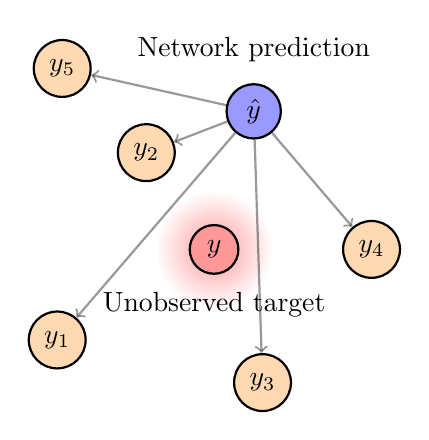
\begin{tikzpicture}
            % Network prediction node
            \node [draw, circle, fill=blue!40, thick] (pred) {\textbf{$\hat{y}$}};
            \node [above=0.15cm] at (pred.north) {Network prediction};

            % Clean target node (not directly used, but for reference)
            \node [shade, inner color=red!40, outer color=white, draw=none] (clean_target_halo) at ([xshift=-0.25cm, yshift=-1.5cm]pred.south west) [circle, minimum size=1.5cm] {};
            \node [draw, circle, fill=red!40, thick] (clean_target) at (clean_target_halo)  {\textbf{$y$}};
            \node [below=0.1cm] at (clean_target.south) {Unobserved target};

            % Multiple noisy targets
            \foreach \i/\angle/\distance in {1/210/2.3, 2/125/1.5, 3/290/1.8, 4/0/2, 5/130/3} {
                \node[draw, circle, fill=orange!30, thick] (noisy\i) at ($(clean_target) + (\angle:\distance)$) {\textbf{$y_{\i}$}};
                \draw[->, thick, opacity=0.4] (pred) -- (noisy\i);
            }
        \end{tikzpicture}
    \caption{Illustration of the Noise2Noise framework where a neural network is trained to map a noisy input image to multiple noisy target images representing different realizations of the same underlying clean image.}
    \label{fig:noise2noise}
\end{figure}

\subsection{Specific settings for Noise2Noise}

\paragraph{MSE loss case}

\begin{proposition}
    \label{prop:noise2noise_l2}
    Minimizing \eqref{eq:n2n_loss} with $\rho(x, y) = \| x - y \|_2^2$ gives the same estimator as minimizing \eqref{eq:supervised_loss} as $N \to \infty$ under the following conditions :
    \begin{itemize}
        \item $Y^{(1)}$ and $Y^{(2)}$ are independent given the clean image $X$ (i.e. $Y^{(1)} | X \independent Y^{(2)} | X$).
        \item Noise is centered, i.e. $\mathbb{E}[Y^{(j)} | X^{(j)} = x] = x$ for $j = 1, 2$.
    \end{itemize}
\end{proposition}

\begin{proof}
    We expand the Noise2Noise empirical risk as follows :
    \begin{align*}
        R_{N,1}^{n2n}(\theta) &= \frac{1}{N} \sum_{i=1}^N \left[ \| f_\theta(Y_i^{(1)}) - (X^{(i)} + B^{(2)}) \|_2^2 \right] \\
        &= \frac{1}{N} \sum_{i=1}^N \left[ \|( f_\theta(Y_i^{(1)}) - X^{(i)}) - B^{(2)} \|_2^2 \right] \\
        &= R_{N,1}^{clean}(\theta) + \frac{1}{N} \sum_{i=1}^N \left[ \| B^{(2)} \|_2^2 \right] - \frac{2}{N} \sum_{i=1}^N \left[ (f_\theta(Y_i^{(1)}) - X^{(i)})^T B^{(2)} \right]
    \end{align*}
    However, $\frac{2}{N} \sum_{i=1}^N \left[ (f_\theta(Y_i^{(1)}) - X^{(i)})^T B^{(2)} \right] \xrightarrow[N \to \infty]{a.s.} 2 \mathbb{E} \left[ (f_\theta(Y^{(1)}) - X)^T B^{(2)} \right]$ by the law of large numbers. This expectation vanishes under the independence and zero-mean assumptions on the noise.
    Thus, we have :
    \begin{equation*}
        R_{N,1}^{n2n}(\theta) = R_{N,1}^{clean}(\theta) + \frac{1}{N} \sum_{i=1}^N \left[ \| B^{(2)} \|_2^2 \right] + o(1)
    \end{equation*}
    We show a similar result for the second term of the Noise2Noise empirical risk by swapping $Y^{(1)}$ and $Y^{(2)}$ and we get the following result :
    \begin{equation*}
        R_{N}^{n2n}(\theta) = 2 R_{N}^{clean}(\theta) + \frac{1}{N} \sum_{i=1}^N \left[ \| B_i^{(1)} \|_2^2 + \| B_i^{(2)} \|_2^2 \right] + o(1)
    \end{equation*}
    where we are left with the standard clean denoising empirical risk with its underlying bias and variance decomposition, and an irreductible noise variance term which has no influence as it is independent of $\theta$.
\end{proof}

\subsubsection{MSE Noise2Noise loss for aggregated outputs}

The use of the MSE loss function enables the use of an even more suited training objective for the case of aggregated outputs.
The two independant noisy observations may be obtained by splitting the data into two
different subsets, hence the noise in each subset is higher than the noise in the original data.
This is the case for example in the medical field.
\cite{wu19} propose a consensus loss to alleviate this issue and improve the results of the aggregated outputs 
\begin{equation}
    \hat{y_i} = \frac{1}{2}(f_\theta(y_i^{(1)}) + f_\theta(y_i^{(2)}))
\end{equation}

We start by stating that the supervised loss of the aggregated output can be written as follows :

\begin{align*}
    \mathcal{L}_{\text{clean}}(\theta) &= \frac{1}{N} \sum_{i=1}^N \| \frac{1}{2}(f_\theta(y_i^{(1)}) + f_\theta(y_i^{(2)})) -  x_i \|_2^2 \\
    &= \frac{1}{N} \sum_{i=1}^N \frac{1}{2} \| f_{\theta}(y_i^{(1)}) - x_i \|_2^2 + \frac{1}{2} \| f_{\theta}(y_i^{(2)}) - x_i \|_2^2 - \frac{1}{4} \| f_{\theta}(y_i^{(1)}) - f_{\theta}(y_i^{(2)}) \|_2^2
\end{align*}

Theorem \ref{prop:noise2noise_l2} shows that the the unobserved clean image $x_i$ can be replaced by one of its noisy version $y_i^{(j)}$ in the previous expression without changing the optimal solution of the problem.
Thus, we can rewrite the supervised loss of the aggregated output as follows :

\begin{equation}
    \mathcal{L}_{\text{consensus}}(\theta) = \frac{1}{N} \sum_{i=1}^N \frac{1}{2} \| f_{\theta}(y_i^{(1)}) - y_i^{(2)} \|_2^2 + \frac{1}{2} \| f_{\theta}(y_i^{(2)}) - y_i^{(1)} \|_2^2 - \frac{1}{4} \| f_{\theta}(y_i^{(1)}) - f_{\theta}(y_i^{(2)}) \|_2^2
    \label{eq:consensus_loss}
\end{equation}

\paragraph{Poisson negative log-likelihood case}
\label{sec:noise2noise_poisson}

As we have a strong interest in PET imaging, we will also focus on the case of Poisson noise which is the best model for PET data and other photon-limited imaging modalities.

\begin{definition}
    For two random variables $X: \Omega \to \mathcal{X}$ and $Y: \Omega \to \mathcal{Y}$, we say that $Y \,|\, X \sim \text{Poisson}(X)$ if :
    \begin{equation*}
        \forall i = 1 \dots d, \quad \mathbb{P}(Y[i] = k \,|\, X[i] = x[i]) = \frac{(x[i])^k e^{-x[i]}}{k!}, \quad k \in \mathbb{N}
    \end{equation*}
\end{definition}

\begin{proposition}
    Under the assumption $Y \,|\, X \sim \text{Poisson}(X)$, we have :
    \begin{equation*}
        \mathbb{E}[Y \,|\, X] = X
    \end{equation*}
\end{proposition}

\begin{proof}
    By definition of the Poisson distribution, we have :
    \begin{align*}
        \mathbb{E}[Y[i] \,|\, X[i] = x[i]] &= \sum_{k=0}^{\infty} k \cdot \mathbb{P}(Y[i] = k \,|\, X[i] = x[i]) \\
        &= \sum_{k=0}^{\infty} k \cdot \frac{(x[i])^k e^{-x[i]}}{k!} \\
        &= x[i] \sum_{k=1}^{\infty} \frac{(x[i])^{k-1} e^{-x[i]}}{(k-1)!} \\
        &= x[i] \cdot 1 = x[i]
    \end{align*}
    Thus, we have $\mathbb{E}[Y \,|\, X] = X$.
\end{proof}

Now, we consider the case of Poisson noise (i.e. $Y^{(j)} \,|\, X^{(j)} \sim \text{Poisson}(X^{(j)}), \quad j = 1, 2$).
Given a clean image $x$ and a noisy observation $y$ corrupted by Poisson noise, the likelihood of observing $y$ given $x$ is given by :
\begin{equation*}
    p(y|x) = \prod_{i} \frac{(x[i])^{y[i]} e^{-x[i]}}{y[i]!}
\end{equation*}
Taking the negative logarithm of this likelihood gives us the Poisson negative log-likelihood loss as defined in the following definition.

\begin{definition}
    The Poisson negative log-likelihood loss between two images $y$ and $x$ is defined as follows :
    \begin{equation*}
        \mathcal{L}_{Poisson}(y, x) = \sum_{i} \left[ y[i] - x[i] \log(y[i]) + \log(x[i]!) \right]
    \end{equation*}
\end{definition}

\begin{proposition}
    \label{prop:noise2noise_poisson}
    If $Y | X=x \sim \text{Poisson}(x)$, then minimizing \eqref{eq:n2n_loss} with $\rho = \mathcal{L}_{Poisson}$ gives the same estimator as minimizing \eqref{eq:supervised_loss} as $N \to \infty$ under the following conditions :
    \begin{itemize}
        \item $Y^{(1)}$ and $Y^{(2)}$ are independent given the clean image $X$ (i.e. $Y^{(1)} | X \independent Y^{(2)} | X$)..
    \end{itemize}
\end{proposition}

\begin{proof}
    The poisson negative log-likelihood between $Y_1$ and $Y_2$ can be expressed as follows :
    \begin{equation*}
        \mathcal{L}_{Poisson}(Y_1, Y_2) = Y_1 - Y_2 \log(Y_1) + \log(Y_2!)
    \end{equation*}
    We expand the Noise2Noise Poisson empirical risk as follows :
    \begin{align*}
        R_{N,1}^{n2n}(\theta) &= \frac{1}{N} \sum_{i=1}^N \left[ \mathcal{L}_{Poisson}(f_\theta(Y_i^{(1)}), Y_i^{(2)}) \right] \\
        &= \frac{1}{N} \sum_{i=1}^N \left[ f_\theta(Y_i^{(1)}) - Y_i^{(2)} \log(f_\theta(Y_i^{(1)})) + \log(Y_i^{(2)}!) \right]
    \end{align*}
    Yet, $\frac{1}{N} \sum_{i=1}^N Y_i^{(2)} \log(f_\theta(Y_i^{(1)})) \xrightarrow[N \to \infty]{a.s.} \mathbb{E} \left[ Y^{(2)} \log(f_\theta(Y^{(1)})) \right]$ due to the law of large numbers. Under the independence assumption on the noise, this expectation can be rewritten as 
    \begin{align*}
        \mathbb{E} \left[ Y^{(2)} | X \right] \mathbb{E} \left[ \log(f_\theta(Y^{(1)})) \right] = X \mathbb{E} \left[ \log(f_\theta(Y^{(1)})) \right]
    \end{align*}
    Then, the empirical risk satisfies the following almost sure convergence :
    \begin{align*}
        R_{N,1}^{n2n}(\theta) \xrightarrow[N \to \infty]{a.s.} \mathbb{E} \left[ f_\theta(Y^{(1)}) - X \log(f_\theta(Y^{(1)})) + \log(Y^{(2)}!) \right]
    \end{align*}
    We can do the same for the second term of the loss by swapping $Y^{(1)}$ and $Y^{(2)}$ and we get the following result :
    \begin{equation*}
        R_{N}^{n2n}(\theta) \xrightarrow[N \to \infty]{a.s.} 2 \mathbb{E} \left[ f_\theta(Y) - X \log(f_\theta(Y)) + \log(Y!)\right]
    \end{equation*}
    where we are left with the standard clean poisson negative-log likelihood risk plus a constant term independent of $\theta$.
\end{proof}

\subsection{General Noise2Noise theory}

In proofs of Proposition \ref{prop:noise2noise_l2} and \ref{prop:noise2noise_poisson}, we can see that the empirical risks of the Noise2Noise loss functions are asymptotically the same
up to an additional term independent of the parameters $\theta$ to be optimized, hence leading to the same optimal solution.
In this section, we try to give more general theoretical insights to understand the Noise2Noise framework and its guarantees.
The choice of the loss function $\rho$ is crucial to ensure those guarantees and we will see that the noise model also plays a key role in the effectiveness of the Noise2Noise framework.

\subsubsection{Noise-induced loss bias}

\begin{definition}
    We define the noise-induced loss bias as between two vectors $z$ and $x$ as the difference between the expected value of the loss function $\rho$ evaluated at $z$ and a noisy observation $Y$ and the actual distance between $z$ and $x$, i.e. :
    \begin{equation}
        \Delta_\rho(z, x) = \mathbb{E}[\rho(z, Y) | X=x] - \rho(z, x)
    \end{equation}
\end{definition}

We denote as $R^{\text{N2N}}(\theta)$ (resp. $R^{\text{clean}}(\theta)$) the expected value of the Noise2Noise loss (resp. the supervised loss) over the distribution of the noisy observations.

\begin{equation}
    R^{\text{N2N}}(\theta) = \mathbb{E}_{X, Y^{(1)}, Y^{(2)}}[\rho(f_\theta(Y^{(1)}), Y^{(2)})]
\end{equation}

\begin{equation}
    R^{\text{clean}}(\theta) = \mathbb{E}_{X, Y}[\rho(f_\theta(Y), X)]
\end{equation}

\begin{proposition}
    The Noise2Noise and the supervised expected risks are tied by the following relation :
    \begin{equation}
        R^{\text{N2N}}(\theta) = R^{\text{clean}}(\theta) + \mathbb{E}[\Delta_\rho(f_\theta(Y), X)]
    \end{equation}
\end{proposition}

\begin{proof}
    We have :
    \begin{align*}
        R^{\text{N2N}}(\theta) &= \mathbb{E}_{X, Y^{(1)}, Y^{(2)}}[\rho(f_\theta(Y^{(1)}), Y^{(2)})] \\
        &= \mathbb{E}_{X, Y^{(1)}}[\mathbb{E}_{Y^{(2)}}[\rho(f_\theta(Y^{(1)}), Y^{(2)}) | X, Y^{(1)}]] \\
        &= \mathbb{E}_{X, Y^{(1)}}[\mathbb{E}_{Y^{(2)}}[\rho(f_\theta(Y^{(1)}), Y^{(2)}) | X]]
    \end{align*}
    Let $z = f_\theta(Y^{(1)})$, we have $\mathbb{E}_{Y^{(2)}}[\rho(z, Y^{(2)}) | X] = \rho(z, X) + \Delta_\rho(z, X)$ by definition of the noise-induced loss bias. Thus, we have :
    \begin{align*}
        R^{\text{N2N}}(\theta) &= \mathbb{E}_{X, Y^{(1)}}[\rho(f_\theta(Y^{(1)}), X) + \Delta_\rho(f_\theta(Y^{(1)}), X)] \\
        &= R^{\text{clean}}(\theta) + \mathbb{E}[\Delta_\rho(f_\theta(Y), X)]
    \end{align*}
\end{proof}

The $\mathbb{E}[\Delta_\rho(f_\theta(Y), X)]$ term is very informative regarding the effectiveness of the Noise2Noise framework for a given noise model and loss function.
If this term is independent of the parameters $\theta$, then minimizing the Noise2Noise loss is equivalent to minimizing the supervised loss and we can learn to denoise without ever observing clean images.

\begin{corollary}
    \label{coro:delta}
    The minimization of $R^{\text{N2N}}(\theta)$ yields the same parameters as the minimization of $R^{\text{clean}}(\theta)$ if and only if $\Delta_\rho(z, x)$ is independent of $z$.
\end{corollary}

\subsubsection{Noise2Noise for centered noise}

\begin{definition}
    We say that a noise model is centered if the expected value of the noisy observation $Y$ given the clean image $X=x$ is equal to $x$, i.e. $\mathbb{E}[Y | X=x] = x$.
\end{definition}

\begin{proposition}
    \label{prop:noise2noise_centered_mse}
    If the noise is centered, i.e. $\mathbb{E}[Y | X=x] = x$, then minimizing the Noise2Noise loss with the MSE loss function is equivalent to minimizing the supervised loss as $N \to \infty$.
\end{proposition}

\begin{proof}
If the MSE loss function is used, the noise-induced loss bias is calculated as follows :
\begin{align*}
    \Delta_\rho(z, x) &= \mathbb{E}[\| z - Y \|_2^2 | X=x] - \| z - x \|_2^2 \\
    &= \mathbb{E}[\| z - x + (x - Y) \|_2^2 | X=x] - \| z - x \|_2^2 \\
    &= \mathbb{E}[\| z - x \|_2^2 + \| x - Y \|_2^2 + 2 \langle z - x, x - Y \rangle | X=x] \\
    &\quad - \| z - x \|_2^2 \\
    &= \mathbb{E}[\| x - Y \|_2^2 | X=x] + 2 \langle z - x, \mathbb{E}[x - Y | X=x] \rangle
\end{align*}
According to corollary \ref{coro:delta}, we need this quantity to be independent of $z$. Thus, we need the term $\langle z - x, \mathbb{E}[x - Y | X=x] \rangle$ to vanish for all $z$, which is equivalent to having $\mathbb{E}[Y | X=x] = x$.
\end{proof}

Note that we recover the result of Proposition \ref{prop:noise2noise_l2} in the case of additive centered noise and the MSE loss function.
We have proven that the Noise2Noise framework, combined with the use of the MSE loss function, is valid for any noise model as long as the noise is centered around its clean counterpart,
in addition to the independence assumption between the two noisy observations given the clean image.
For example, if $Y|X=x$ follows a log-normal distribution, then $\mathbb{E}[Y|X=x] = x \exp(\sigma^2/2) \neq x$ and the Noise2Noise framework with the MSE loss function is not valid in this case.

\subsubsection{Toward the exponential family of distributions}
As we already saw in the case of the MSE loss under gaussian noise and the Poisson negative log-likelihood loss under Poisson noise, the additional term $\mathbb{E}[\Delta_\rho(f_\theta(Y), X)]$ is respectively equal to the variance of the noise and a constant term independent of $\theta$.
We can show that this property can be extended under some asumptions to the exponential family of distributions and for the corresponding negative log-likelihood loss function.
\begin{definition}
    A distribution belongs to the exponential family if its probability density function can be written as :
    \begin{equation}
        p(y|x) = h(y) \exp(\langle T(y), \eta(x) \rangle - \phi(x))
    \end{equation}
    where $T(y)$ is the sufficient statistic, $\eta(x)$ is the natural parameter, $\phi(x)$ is the log-partition function and $h(y)$ is the base measure.
\end{definition}
Using the exponential family formalism, we can write the negative log-likelihood loss function as follows :
\begin{equation}
    \rho(z, y) = -\log p(y|z) = -\log h(y) - \langle T(y), \eta(z) \rangle + \phi(z)
\end{equation}
Then, computing the noise-induced loss bias gives us :
\begin{align*}
    \Delta_\rho(z, x) &= \mathbb{E}[\rho(z, Y) | X=x] - \rho(z, x) \\
    &= \mathbb{E}[-\log h(Y) - \langle T(Y), \eta(z) \rangle + \phi(z) | X=x] - (-\log h(x) - \langle T(x), \eta(z) \rangle + \phi(z)) \\
    &= \mathbb{E}[-\log h(Y) | X=x] + \log h(x) - \langle \mathbb{E}[T(Y) | X=x] - T(x), \eta(z) \rangle + \phi(z) - \phi(z) \\
    &= \mathbb{E}[-\log h(Y) | X=x] + \log h(x) - \langle \mathbb{E}[T(Y) | X=x] - T(x), \eta(z) \rangle
\end{align*}
For this quantity to be independent of $z$, we need the term $\langle \mathbb{E}[T(Y) | X=x] - T(x), \eta(z) \rangle$ to vanish, which is equivalent to having $\mathbb{E}[T(Y) | X=x] = T(x)$, hence Proposition \ref{prop:ef_n2n}.
\begin{proposition}
    \label{prop:ef_n2n}
    For a noise model belonging to the exponential family, if the sufficient statistic $T(Y)$ is an unbiased estimator of $T(X)$, then minimizing the Noise2Noise loss with the corresponding negative log-likelihood loss function is equivalent to minimizing the supervised loss as $N \to \infty$.
\end{proposition}
Note that this property of the sufficient statistics is satisfied for Gaussian and Poisson distributions as we have already seen in Proposition \ref{prop:noise2noise_l2} and \ref{prop:noise2noise_poisson}
but also for other distributions like the Bernoulli distribution, the Exponential distribution, or the Gamma distribution.
On the other hand, the log-normal distribution belongs to the exponential family but its sufficient statistic is $T(Y) = (\log Y, (\log Y)^2)$.
$\mathbb{E}[\log Y | X=x] = \log x - \frac{\sigma^2}{2}$ and $\mathbb{E}[(\log Y)^2 | X=x] = (\log x)^2 + \sigma^2 - \sigma^2 \log x + \frac{\sigma^4}{4}$, hence the sufficient statistic is not an unbiased estimator of $T(X) = (\log X, (\log X)^2)$.

\subsubsection{Empirical Noise2Noise}

The two previous paragraphs show that neither the MSE loss function nor the log-normal negative log-likelihood loss function are appropriate for the Noise2Noise framework under log-normal noise.
For log-normal distributions or any other noise model that doesn't satisfy either the centered noise assumption or the sufficient statistic unbiasedness assumption,
we can empirically observe that the Noise2Noise framework will indeed tend to denoise the images but will not converge to the supervised solution as the number of training samples increases.
In such cases, we lack interpretability as the resulting estimator is no longer the optimal solution of a well-defined supervised loss function or even a MMSE estimator in some cases.

\subsubsection{Particular case of the MAE loss}

The Minimum Absolute Error (MAE) loss function is defined as $\rho(z, y) = \| z - y \|_1$ is a special case or the Noise2Noise framework.
Its noise-induced loss bias is given by $\Delta_\rho(z, x) = \mathbb{E}[\| z - Y \|_1 | X=x] - \| z - x \|_1$.
If $g_x(z) = \mathbb{E}[\| z - Y \|_1 | X=x]$, then $g_x'(z) = 2 \mathbb{P}(Y \leq z | X=x) - 1 = 2 F_{Y|X=x}(z) - 1$ where $F_{Y|X=x}$ is the cumulative distribution function of $Y$ given $X=x$.
In order to apply Corollary \ref{coro:delta}, we need $g_x'(z) = 0$ for all $z$, which is equivalent to having $F_{Y|X=x}(z) = 1/2$ for all $z$, which is impossible.
Thus, the MAE loss function is not appropriate for the Noise2Noise framework ; whereas the supervised loss with the MAE loss function will converge to the conditional median of $Y$ given $X=x$, the Noise2Noise loss will not converge to any well-defined estimator.

\subsection{Extension to Bregman Geometry}

\subsubsection{Bregman Geometry}

In this section, we study the potential Noise2Noise guarantees in the context of Bregman geometry, which is a generalization of the Euclidean geometry, the MSE loss function or any other loss function that can be expressed as a Bregman divergence.
\begin{definition}
Let $\phi: \mathbb{R}^d \to \mathbb{R}$ be a strictly convex and differentiable function. The Bregman divergence associated with $\phi$ is defined as :
\begin{equation}
    \label{bregman_divergence}
    D_\phi(z, y) = \phi(z) - \phi(y) - \langle \nabla \phi(y), z - y \rangle
\end{equation}
\end{definition}
\noindent The Bregman divergence is not a distance in the mathematical sense as it is not symmetric and does not satisfy the triangle inequality, but it is a measure of dissimilarity between two points in the space defined by $\phi$.
It is though positive and vanishes if and only if $z = y$.
Note that the MSE loss function is a special case of the Bregman divergence with $\phi(z) = \| z \|_2^2$ and that the Poisson negative log-likelihood loss function is also a special case of the Bregman divergence with $\phi(z) = \sum_i z[i] \log z[i] - z[i]$.

Due to our conventions, the $z$ argument denotes the prediction and the $y$ argument denotes the target.
As the two variables are not symmetric in the Bregman divergence definition, we can swap the role played by $z$ and $y$ to get a different interpretation of the Bregman divergence.
In the target-first case, we have :
\begin{align*}
    \nabla_z \mathbb{E}[D_\phi(Y, z) | X=x] &= \nabla_z \mathbb{E}[\phi(Y) - \phi(z) - \langle \nabla \phi(z), Y - z \rangle | X=x] \\
    &= \nabla^2 \phi(z) \left( z - \mathbb{E}[Y | X=x] \right)
\end{align*}
Therefore, under strict convexity of $\phi$, the minimizer of $\mathbb{E}[D_\phi(Y, z) | X=x]$ is given by $z^* = \mathbb{E}[Y | X=x]$.
The target-first Bregman loss elicits the conditional mean of $Y$ given $X=x$. The same reasoning gives for the prediction-first Bregman loss :
\begin{align*}
    \nabla_z \mathbb{E}[D_\phi(z, Y) | X=x] &= \nabla_z \mathbb{E}[\phi(z) - \phi(Y) - \langle \nabla \phi(Y), z - Y \rangle | X=x] \\
    &= \nabla \phi(z) z - \mathbb{E}[\nabla \phi(Y) Y | X=x]
\end{align*}
which yields the minimizer $z^* = (\nabla \phi)^{-1}(\mathbb{E}[\nabla \phi(Y) | X=x])$, hence the quasi-arithmetic mean in the transformed space defined by $\nabla \phi$.
We can now state the following propositions regarding the Noise2Noise framework in the context of Bregman geometry.

\begin{proposition}
    \label{prop:b_target_first}
    If noise is centered, i.e. $\mathbb{E}[Y | X=x] = x$, then minimizing the Noise2Noise loss with a \textbf{target-first} Bregman divergence yields the same estimator as minimizing the supervised loss as $N \to \infty$.
\end{proposition}
\begin{proof}
    We derive the noise-induced loss bias in the context of Bregman geometry with target-first Bregman divergence :
    \begin{align*}
        \Delta_\rho(z, x) &= \mathbb{E}[D_\phi(Y, z) | X=x] - D_\phi(x, z) \\
        &= \mathbb{E}[\phi(Y) - \phi(z) - \langle \nabla \phi(z), Y - z \rangle | X=x] - (\phi(x) - \phi(z) - \langle \nabla \phi(z), x - z \rangle) \\
        &= \mathbb{E}[\phi(Y) | X=x] - \phi(x) + \langle \nabla \phi(z), x - \mathbb{E}[Y | X=x] \rangle
    \end{align*}
The term in $z$ vanishes as $\mathbb{E}[Y | X=x] = x$.
\end{proof}
\noindent Proposition \ref{prop:b_target_first} states that any target-first Bregman divergence suits the Noise2Noise framework, but the performance of the resulting estimator will depend on the choice of the Bregman divergence which has to be adapted to the noise model.
\begin{proposition}
    Minimizing the Noise2Noise loss with a \textbf{prediction-first} Bregman divergence yields the same estimator as minimizing the supervised loss as $N \to \infty$ if and only if :
    \begin{equation}
        \label{prop:b_prediction_first}
        \mathbb{E}[\nabla \phi(Y) | X=x] = \nabla \phi(x)
    \end{equation}
    If we also assume that the noise is centered, i.e, $\mathbb{E}[Y | X=x] = x$, then this condition is equivalent to $\phi$ being a quadratic function :
    \begin{equation}
        \phi(z) = \frac{1}{2} z^T Q z + b^T z + c
    \end{equation}
    with $Q$ a positive definite matrix, $b \in \mathbb{R}^d$ and $c \in \mathbb{R}$.
\end{proposition}

\begin{proof}
We derive the noise-induced loss bias in the context of Bregman geometry with prediction-first Bregman divergence :
\begin{align*}
    \Delta_\rho(z, x) &= \mathbb{E}[D_\phi(z, Y) | X=x] - D_\phi(z, x) \\
    &= \mathbb{E}[\phi(z) - \phi(Y) - \langle \nabla \phi(Y), z - Y \rangle | X=x] - (\phi(z) - \phi(x) - \langle \nabla \phi(x), z - x \rangle) \\
    &= -\mathbb{E}[\phi(Y) | X=x] + \phi(x) - \mathbb{E}[\langle \nabla \phi(Y), z - Y \rangle | X=x] + \langle \nabla \phi(x), z - x \rangle
\end{align*}
Let $g_x(z) = \mathbb{E}[\langle \nabla \phi(Y), z - Y \rangle | X=x] - \langle \nabla \phi(x), z - x \rangle$, we have $g_x'(z) = \mathbb{E}[\nabla \phi(Y) | X=x] - \nabla \phi(x)$.
In order to apply Corollary \ref{coro:delta}, we need $g_x'(z) = 0$ for all $z$, which is equivalent to $\mathbb{E}[\nabla \phi(Y) | X=x] = \nabla \phi(x)$.
It remains to be shown that this condition is equivalent to the gradient of $\phi$ being affine.
If noise is centered, then we can write $\mathbb{E}[\nabla \phi(Y) | X=x] = \nabla \phi(\mathbb{E}[Y | X=x])$.
We denote $g(z) = \nabla \phi(z)$, then the condition becomes $g(\mathbb{E}[Y | X=x]) = \mathbb{E}[g(Y) | X=x]$.
If $g$ is affine, the result is immediate. Conversely, if the condition holds for all $x$, then we can write $g(\mathbb{E}[Y | X=x]) = \mathbb{E}[g(Y) | X=x]$ for any random variable $Y$ with finite expectation.
For a two-point distribution $Y \sim p \delta_{y_1} + (1-p) \delta_{y_2}$, we have $\mathbb{E}[Y] = p y_1 + (1-p) y_2$ and $\mathbb{E}[g(Y)] = p g(y_1) + (1-p) g(y_2)$, hence $g(p y_1 + (1-p) y_2) = p g(y_1) + (1-p) g(y_2)$ for all $y_1, y_2$ and $p \in [0, 1]$, which is the definition of an affine function.
By integrating, we obtain that $\phi(x) = \frac{1}{2} x^T Q x + b^T x + c$ and the strict convexity of $\phi$ implies that $Q$ is positive definite.
\end{proof}

\subsubsection{Mahalanobis distance and correlated noise}

Proposition \ref{prop:b_prediction_first} can be interpreted as a generalization of the MSE loss function to the case of correlated noise.
Plugging $\phi(z) = \frac{1}{2} z^T Q z$ into the Bregman divergence definition \eqref{bregman_divergence} gives us :
\begin{align}
    D_\phi(z, y) &= \frac{1}{2} z^T Q z - \frac{1}{2} y^T Q y - \langle Q y, z - y \rangle \\
    &= \frac{1}{2} z^T Q z - \frac{1}{2} y^T Q y - y^T Q z + y^T Q y \\
    &= \frac{1}{2} (z - y)^T Q (z - y)
\end{align}
\noindent which is the Mahalanobis distance between $z$ and $y$ with respect to the positive definite matrix $Q$.
This is basically a generalization of Proposition \ref{prop:noise2noise_centered_mse}.
This means that any weighted MSE loss function with a positive definite weight matrix $Q$ is appropriate for the Noise2Noise framework under centered noise.
This has some potential benefits in the case of correlated noise where the covariance matrix of the noise is not diagonal, as the Mahalanobis distance can be used to decorrelate the noise and improve the denoising performance.
One can also choose diagonal weights to give more importance to some pixels than others, for example in the case of a region of interest in the image or sensitivity maps in medical imaging.




% \subsection{Other Noise2Noise-based frameworks}


% \subsubsection{Noise2Noise}

% In the context of a known noise model, the Noise2Noise principle can be extended to approaches like \textbf{Noisier2Noise} \cite{moran_noisier2noise_2019} where we can add extra noise to a single noisy image to create a pair of noisy images with a lower noise level in the target image.

% \subsubsection{Noise2Score}

% \cite{kim_noise2score_nodate} propose a 2-step framework called \textbf{Noise2Score}. First the score function is being estimated using a DAE trained under framework closed to Noisier2Noise where noise is embedded into the images according to the noise model and then the network learn the mapping to retrieve less noisy images.
% Then, the estimated denoised images are simply computed using the appropriate Tweedie's formula variant.
% This method is very promissing at it is at the crossroad between bayesian methods with strong mathematical background and self-supervised learning.


% \subsubsection{Noise2NoiseFlow}

% \cite{maleky_noise2noiseflow_2022} propose a framework at the crossroad between density estimation and the Noise2Noise framework. Density estimation is performed using Noise Flow \cite{abdelhamed_noise_2019}, a normalizing flow model designed to learn complex noise distributions from data.
% Notice that the density is closely related to the score.
% Whereas classical score matching methods require model trained in a supervised manner with clean data or denoising auto-encoders trained in an unsupervised manner to estimate the score function, they propose to directly learn the score function from noisy data only using the Noise2Noise principle.
% Both the denoising model and the normalizing flow are trained jointly using pairs of noisy images under the following loss function :

% \begin{equation}
%     \mathcal{L}(\theta, \phi) =  \underset{\substack{y_1, y_2 \sim p_{noisy}}}{\mathbb{E}} \left[ - \log p_{N_\phi}(y_1 | f_\theta(y_2)) - \log p_{N_\phi}(y_2 | f_\theta(y_1)) \right] + \lambda \mathcal{L}_{n2n}(\theta)
% \end{equation}

% with $p_{N_\phi}$ being the noise distribution modeled by the normalizing flow with parameters $\phi$, $f_\theta$ the denoising model with parameters $\theta$ and $\mathcal{L}_{n2n}(\theta)$ the standard Noise2Noise loss. The authors of Noise2NoiseFlow show that this additional term gives more stability to the training process and leads to better denoising results.

% Note that this framework is useless if we already know the natural noise distribution in the data as we could directly use it to denoise images using bayesian methods.

\section{Bootstrapping noisy measurements}

In this section, we discuss how to generate two independant measurements to apply Noise2Noise on from a single measurement.

\subsection{Statistical bootstrapping}

In the context of additive gaussian noise, \textbf{Recorrupted2Recorrupted} \cite{Pang2021} aims to provide a way to simulate noisy image pairs satisfying statistical conditions from single measurements.
This can be particularly usefull in the case of medical imaging where we often have only one noisy image per patient and where the noise model is well-known.
We propose an intuitive alternative to their method with Poisson noise.

\begin{definition}{Infinitely divisible distribution}
    Let $Y$ be a random variable. $Y$ is said to be $n$-divisible if there exists a sequence of $n$ i.i.d. random variables $\{Y_i\}_{i=1}^n$ such that $Y \stackrel{d}{=} \sum_{i=1}^n Y_i$. If $Y$ is $n$-divisible for all $n \in \mathbb{N}$, then $Y$ is said to be infinitely divisible.
\end{definition}

If the noise model is well-known and satisfies the infinite divisibility property, we can use this property to generate pairs of noisy images from a single noisy image by splitting the noise into two independent parts.

\begin{proposition}
    The Poisson distribution is infinitely divisible ; in particular, it is $2$-divisible. Thus, if $Y \sim \text{Poisson}(\lambda)$, then there exists two i.i.d. random variables $Y_1$ and $Y_2$ such that $Y = Y_1 + Y_2$ and $Y_1, Y_2 \sim \text{Poisson}(\lambda/2)$.
    \label{prop:poisson_divisibility}
\end{proposition}

\begin{proof}
    This proof will focus on the case of $2$-divisibility, but it can be easily extended to the general case of $n$-divisibility.
    Let $Y$ be a random variable following a Poisson distribution with parameter $\lambda$, and let $Y_1 | Y=y \sim \text{Binomial}(y, 1/2)$ be a random variable following a binomial distribution with parameters $y$ and $1/2$ conditionally on $Y=y$. We define $Y_2 = Y - Y_1$. We have the following result for the distribution of $Y_1$ :
    \begin{align*}
        \mathbb{P}(Y_1 = k) &= \sum_{y=k}^{\infty} \mathbb{P}(Y_1 = k | Y = y) \mathbb{P}(Y = y) \\
        &= \sum_{y=k}^{\infty} \binom{y}{k} \left( \frac{1}{2} \right)^y \frac{\lambda^y e^{-\lambda}}{y!} \\
        &= \sum_{y=k}^{\infty} \frac{y!}{k!(y-k)!} \left( \frac{1}{2} \right)^y \frac{\lambda^y e^{-\lambda}}{y!} \\
        &= \frac{1}{k!} \left( \frac{\lambda}{2} \right)^k e^{-\lambda/2} \sum_{y=k}^{\infty} \frac{(\lambda/2)^{y-k} e^{-\lambda/2}}{(y-k)!} \\
        &= \frac{1}{k!} \left( \frac{\lambda}{2} \right)^k e^{-\lambda/2}
    \end{align*}
    Thus, $Y_1$ follows a Poisson distribution with parameter $\lambda/2$. By symmetry, $Y_2$ also follows a Poisson distribution with parameter $\lambda/2$. Moreover, we have $Y = Y_1 + Y_2$ by definition.

    Finally, we show that $Y_1$ and $Y_2$ are independent. We have :
    \begin{align*}
        \mathbb{P}(Y_1 = k, Y_2 = l) &= \mathbb{P}(Y_1 = k, Y_2 = l | Y = k + l) \mathbb{P}(Y = k + l) \\
        &= \binom{k+l}{k} \left( \frac{1}{2} \right)^{k+l} \frac{\lambda^{k+l} e^{-\lambda}}{(k+l)!} \\
        &= \frac{1}{k!} \left( \frac{\lambda}{2} \right)^k e^{-\lambda/2} \cdot \frac{1}{l!} \left( \frac{\lambda}{2} \right)^l e^{-\lambda/2} \\
        &= \mathbb{P}(Y_1 = k) \mathbb{P}(Y_2 = l)
    \end{align*}
\end{proof}

The previous proposition shows that it is possible to perform binomial thinnning on Poisson data in order to generate independant pairs of noisy images.
However, subsampled images expectation is not the same as the original image expectation, as well as noise variance, which means that the signal to noise ratio is higher in the subsampled images than in the original image.

\cite{gr2r} go beyond the additive Gaussian noise model or Poisson noise model and propose a generic formulation for any posterior distribution $p(Y|X)$ that belongs to the exponential family of distributions.
Their implementation in the case of Poisson noise is shown in the following proposition.
We introduce $\gamma$ and $\alpha$ which respectively control the noise model scale factor and the balance between the two measurements $Y_1$ and $Y_2$ :

\begin{equation}
    \begin{cases}
        Y = \gamma Z \\
        Z | X =x \sim \text{Poisson}(\frac{x}{\gamma}) \\
        W | Z = z \sim \text{Binomial}(z, \alpha) \\
        Y_1 = \frac{Y - \gamma W}{1 - \alpha} \\
        Y_2 = \frac{1}{\alpha} Y - \frac{1 - \alpha}{\alpha} Y_1
    \end{cases}
    \label{eq:gr2r}
\end{equation}

\begin{proposition}
    The measurements admits decomposition $Y = (1 - \alpha) Y_1 + \alpha Y_2$ and satisfy the following properties :
    \begin{itemize}
        \item $Y_1$ and $Y_2$ are independent given the clean image $X$.
        \item $\mathbb{E}[Y_1 | X=x] = \mathbb{E}[Y_2 | X=x] = \mathbb{E}[Y | X=x] = x$.
        \item $\mathbb{V}[Y_1 | X=x] = \frac{1}{1 - \alpha} \mathbb{V}[Y | X=x] = \frac{1}{1 - \alpha} x$.
        \item $\mathbb{V}[Y_2 | X=x] = \frac{1}{\alpha} \mathbb{V}[Y | X=x] = \frac{1}{\alpha} x$.
    \end{itemize}
\end{proposition}

\cite{gr2r} propose a generic proof for the previous proposition when the noise distribution is any member of the exponential family of distributions, which includes the Poisson distribution as a special case.

\begin{remark}
    The definition of $Y_1$ and $Y_2$ in \eqref{eq:gr2r} when $\alpha = 0.5$ and $\gamma = 2$ match the one from proposition \ref{prop:poisson_divisibility}.
\end{remark}

\subsection{Data-based bootstrapping}


\textbf{Noise2Void} \cite{krull_noise2void_2019} and \textbf{Noise2Self} \cite{batson_noise2self_nodate} frameworks further extend the idea of training denoising models without clean targets by using only single noisy images.
\cite{batson_noise2self_nodate} introduce the concept of \textit{$\mathcal{J}$-invariant} functions, which are functions that do not depend on certain subsets of their input.
We train a denoising model to be $\mathcal{J}$-invariant by masking certain pixels of the input image and predicting their values based on the surrounding pixels.
The work of \cite{krull_noise2void_2019} implements this idea by randomly masking pixels in the input image during training and using the unmasked pixels to predict the masked ones.
This is called the \textit{blind-spot} strategy and ensures that the model does not learn to simply copy the noisy input to the output, thus learning the identity.

In some applications, it is also possible to take advantage of the acquisition process to generate multiple noisy measurements of the same underlying clean image.
If a signal $y$ is drawn from \eqref{eq:inverse-problem}, it can be splitted into two non-overlapping subsets of measurements $y_1$ and $y_2$ such that

\begin{equation}
    \begin{cases}
        y_1 = A_1 x + b_1 \\
        y_2 = A_2 x + b_2
    \end{cases}
\end{equation}
with $A_1$ and $A_2$ two linear operators inheriting from $A$ and defined accordingly to $y_1$ and $y_2$ and $b_1$ and $b_2$ two noise vectors.

This idea was exploited in the context of Computed Tomography where odd and even projections are separated to get $K$ sinogram subsets \cite{hendriksen_noise2inverse_2020}.
Each resulting sinogram subset is an even more discretized version of the original sinogram, thus even more ill-posed and noisy than the original problem.
They study two different training strategies.
The first one uses the average of the first $K-1$ sinograms as input and the remaining one as target. This strategy is close to the Noise2Self principle.
The second one is the reversed of the first and is closer to the Noisier2Noise strategy as the input will be noisier than the target.


\section{Generalization of Noise2Noise to linear inverse problems}

In this section, we get back to the general framework where $A$ is unspecified.
Let again $\{(Y_i^{(1)}, Y_i^{(2)})\}_{i=1}^N$ be a finite sequence of independant and statistically distributed random variables and $y_i^{(j)} = A_i^{(j)}x_i + b_i^{(j)}$ the observed degraded images.
We also rewrite \ref{eq:inverse-problem} as :
\begin{equation}
    \begin{cases}
        Y^{(j)} | X=x \sim \mathcal{C}(A^{(j)}x), \quad j = 1, 2 \\
        Y^{(j)} = A^{(j)} X + B^{(j)}, \quad j = 1, 2
    \end{cases}
\end{equation}
with $A^{(j)} \in \mathbb{R}^{d \times m}$ two linear operators inheriting from $A$ and defined accordingly to $Y^{(1)}$ and $Y^{(2)}$.


In the context of non-blind estimation, i.e. when $A^{(j)}$ is known, we can optimize a neural network $f_{\theta}$ under the following objective function \cite{xia_training_nodate} :
\begin{equation}
    \mathcal{L}_{swap}(\theta) = \frac{1}{N} \sum_{i=1}^N \left[ \rho(A_i^{(2)} f_{\theta}(y_i^{(1)}) - y_i^{(2)}) + \rho(A_i^{(1)} f_{\theta}(y_i^{(2)}) - y_i^{(1)}) \right]
    \label{eq:xia_swap_loss}
\end{equation}


\begin{theorem}
    Minimizing \ref{eq:n2n_loss} with $\rho(x, y) = \| x - y \|_2^2$ gives the same estimator as minimizing the homologous supervised loss as $N \to \infty$ under Noise2Noise statistical conditions.
\end{theorem}

\subsubsection{MSE loss}

\begin{proof}
    Proof in theorem \ref{th:noise2noise_l2} is still valid as long as we replace $f_{\theta}(Y^{(j)})$ by $Af_{\theta}(Y^{(j)})$. We thus have :
    \begin{align*}
        R_{N}^{n2n}(\theta) &= \frac{1}{N} \sum_{i=1}^N \left[ \| A_i^{(2)} f_{\theta}(Y_i^{(1)}) - Y_i^{(2)} \|_2^2 + \| A_i^{(1)} f_{\theta}(Y_i^{(2)}) - Y_i^{(1)} \|_2^2 \right] \\
        &= 2 R_{N}^{clean}(\theta) + \frac{1}{N} \sum_{i=1}^N \left[ \| B_i^{(1)} \|_2^2 + \| B_i^{(2)} \|_2^2 \right] + o(1)
    \end{align*}
\end{proof}

\subsubsection{Poisson linear inverse problems}

With the conventions of section \ref{sec:noise2noise_poisson}, we now consider the case of linear inverse problems corrupted by Poisson noise :

\begin{equation}
    Y^{(j)} \sim Poisson(A^{(j)} X), \quad j = 1, 2
\end{equation}

\begin{theorem}
    If $Y | X=x \sim \text{Poisson}(Ax)$, then minimizing \ref{eq:n2n_loss} with $\rho = \mathcal{L}_{Poisson}$ gives the same estimator as minimizing the homologous supervised loss as $N \to \infty$ under Noise2Noise statistical conditions.
\end{theorem}

\begin{proof}
    Proof in theorem \ref{th:noise2noise_poisson} is still valid as long as we replace $f_{\theta}(Y^{(j)})$ by $A f_{\theta}(Y^{(j)})$. If we define the empirical risk as :
    \begin{equation*}
        R_{N}^{n2n}(\theta) = \frac{1}{N} \sum_{i=1}^N \left[ \mathcal{L}_{Poisson}(A_i^{(2)} f_{\theta}(Y_i^{(1)}), Y_i^{(2)}) + \mathcal{L}_{Poisson}(A_i^{(1)} f_{\theta}(Y_i^{(2)}), Y_i^{(1)}) \right]
    \end{equation*}
    then we have :
    \begin{equation*}
        R_{N}^{n2n}(\theta) \xrightarrow[N \to \infty]{a.s.} 2 \mathbb{E} \left[ f_\theta(Y) - A X \log(f_\theta(Y)) + \log(Y!)\right]
    \end{equation*}
\end{proof}

\subsection{Splitting strategies}

\subsubsection{Data splitting}

eg tachella, Noise2Inverse

\subsubsection{Statistical splitting}

eg R2R, GR2R

\subsection{Single-operator framework}

There exists a special case of inverse problems where $A^{(1)} = A^{(2)}$ for each training pair.
In this case, the loss function can be simplified as follows :

\begin{equation}
    \mathcal{L}_{\text{swap}}(\theta) = \frac{1}{N} \sum_{i=1}^N \left[ \rho(A_i f_{\theta}(y_i^{(1)}) - y_i^{(2)}) + \rho(A_i f_{\theta}(y_i^{(2)}) - y_i^{(1)}) \right]
\end{equation}

\subsection{Data consistency enforcement}

Eventhough the loss function \ref{eq:xia_swap_loss} is sufficient to guarantee that the optimal solution of the problem is the same as the one of the supervised problem, it does not enforce data-consistency during training, which can lead to suboptimal results.
Indeed, this term is biased toward smoothness as a denoising objective. Thus it can be usefull to add an extra term to the loss function to enforce data-consistency during training \cite{xia_training_nodate} :

\begin{equation}
    \mathcal{L}_{\text{self}} = \frac{1}{N} \sum_{i=1}^N \left[ \rho(A_i^{(1)} f_{\theta}(y_i^{(1)}) - y_i^{(1)}) + \rho(A_i^{(2)} f_{\theta}(y_i^{(2)}) - y_i^{(2)}) \right]
\end{equation}

In the case of inifinite divisibility-based frameworks where $y = y_1 + y_2$ and $y_1$ and $y_2$ are derived from the same probability law, we can simply use the following data-consistency term :

\begin{equation}
    \mathcal{L}_{\text{self}} = \frac{1}{N} \sum_{i=1}^N \rho\left( \frac{A_i f_{\theta}(y_i^{(1)}) + A_i f_{\theta}(y_i^{(2)})}{2} - y\right)
\end{equation}
where we want the resulting average to match the original noisy image $y$.

Eitherway, the final loss function is then written as :
\begin{equation}
    \mathcal{L}_{\text{total}} = \mathcal{L}_{\text{swap}} + \lambda \mathcal{L}_{\text{self}}
\end{equation}
with $\lambda$ a hyperparameter to tune the weight of the data-consistency term.

\newpage
\appendix
\include{sections/appendix/appendix.tex}

% Print the bibliography
\newpage
\printbibliography

\end{document}
